%----------------------------------------------------------------------------
\chapter{Rendszer felépítése}
\label{sec:system}
%----------------------------------------------------------------------------
Ebben a fejezetben szeretném bemutatni az elkészített rendszert és az azt alkotó egyes elemeket.
A fejezet végén részletezésre kerül egy teljes mérés folyamata és a kapott eredmények feldolgozásának lépései.

%----------------------------------------------------------------------------
\section{Rendszer részei}
%----------------------------------------------------------------------------
Az elkészült rendszer három fő komponensből áll. Ezek együttesen képesek tetszőleges tulajdonsággal rendelkező szolgáltatás hálózatokat megvalósítani, azt Kubernetes alatt elindítani, forgalmat generálni és mérés során adatokat gyűjteni. 

Az egyes részekről bővebben is lesz szó, azonban most átfogóan ismertetem a rendszert, ami a \ref{fig:system_overview} ábrán látható. Minden elem megalkotásánál egy lényeges szempont volt, hogy az elkészült rendszerrel könnyen lehessen méréseket indítani és a lehető legtöbb paraméter konfigurálható legyen.

A mérések paramétereit egy konfigurációs fájlban tudjuk megadni, ahonnan egy Python program olvassa be és vezényli le a mérések elvégzését.
Először a Kubernetes API-n keresztül létrehoz egy \textit{ServiceGraph} objektumot, ami nem egy beépített típus.
Az objektum értelmezéséhez és megfelelő kezeléséhez létre kellett hozni egy operátort, ami képes egy ilyen definíció szerint létrehozni a szükséges erőforrásokat (\textit{deployment, pod, service, HPA}).

Az elindításra kerülő kapszulák tartalmaznak egy alkalmazást, amely számára az operátor indításkor át tudja adni szükséges paramétereket. 
A Go nyelven megírt alkalmazás képes a beérkező kéréseket fogadni és az indításkor megadott paraméterek alapján műveletet végrehajtani a hatására.
Elég speciális igényeink vannak az alkalmazást illetően, ezért külön implementálni kellett.

%Ahhoz, hogy az egyes kiszolgáló egységeket is tudjuk tetszés szerint konfigurálni kell egy olyan képfájl, ami a megadott paraméterek alapján tud működni.
%Ezért írni kellett egy külön alkalmazást hozzá.

Miután elkészültek a kért objektumok és képesek már kiszolgálni a klaszteren kívülről érkező igényeket a Python szkript elkezd számukra forgalmat generálni.
A terhelés lejárta után ki kell nyerni a mérés során keletkezett adatokat.
A feladat elvégzésében segítségünkre lesz a Prometheus\citep{Prometheus} alkalmazás, ami gyűjti és exportálja a klaszterből érkező metrikákat. 

Az elkészült rendszerhez szükséges részek forráskódjai megtalálhatóak a GitHub felületén\citep{gitRepo}. 

% Rendszer áttekintése -------------------------------------------------------
\begin{figure}[!ht]
\centering
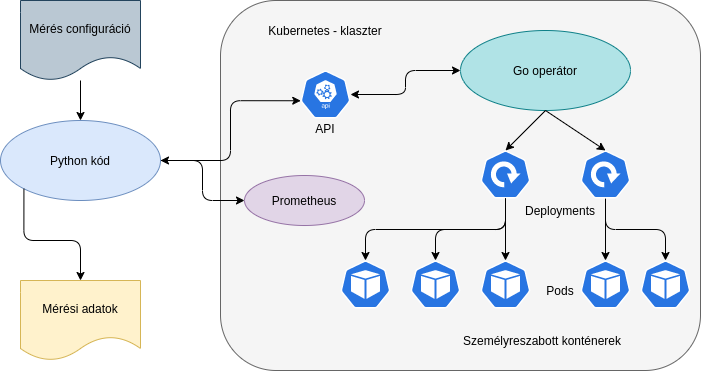
\includegraphics[width=150mm, keepaspectratio]{figures/system_overview.png}
\caption{Rendszer áttekintése}
\label{fig:system_overview}
\end{figure}

%----------------------------------------------------------------------------
\section{Korábbi munkák}
%----------------------------------------------------------------------------
A korábbi projekttárgyak keretén belül már foglalkoztam hasonló kérdéskörrel, így már volt az egyes eszközök használatához tapasztalat és implementáció is, amiből ki lehetett indulni. 
Önálló labor tárgyban megismerkedtem a Go programozási nyelvvel, és elkészítettem egy Kubernetes operátort, ami képes egyedi erőforrás definíciók feldolgozására és ez alapján képes beépített objektumokat létrehozni.
A félév elején ezt tovább kellett bővíteni, hogy képes legyen skálázót is létrehozni valamint javítani kellett a megbízhatóságán is.

Korábbi tanulmányaim során elkezdtem készíteni egy Go nyelven íródott alkalmazást, melynek célja azonos volt a mostani projektben foglalttal.
A megkezdett alkalmazás is egy kellően szabadon konfigurálható paraméterezéssel rendelkező webszerver volt, hogy tetszőleges módon tudja kiszolgálni a beérkező kéréseket. 
A korábbi állományból kiindulva kellett fejleszteni a funkcionalitásán, hogy valósághűbb eredményeket tudjon szolgáltatni.

%----------------------------------------------------------------------------
\section{Operátor}
%----------------------------------------------------------------------------
Fontos szempontnak tekintettük, hogy egyszerű konfigurációs fájl alapján létre lehessen hozni a szolgáltatáshálót, amit szeretnénk tesztelni.
A Kubernetes rendszer nem tartalmaz olyan erőforrást, ami számunkra ezt a funkcionalitást alapvetően támogatná.
A feladat számunkra az lesz, hogy egy közös konfiguráció alapján több különböző fajta, már beépített erőforrást hozzunk létre.
Már az orkesztrációs platform fejlesztésénél felkészültek arra az esetre, hogy sok egyedi igény fog megjelenni a különböző használatból fakadóan, ezért már fejlesztés közben fontos szempont volt a Kubernetes könnyű kibővítése.
A mögöttes gondolat az, hogy nagyon változó igények és funkcionalitások jelenhetnek meg a felhasználási körülményektől függően, amiket nem célszerű a központi egységbe implementálni, hiszen akkor a rendszer könnyen átláthatatlanná és inkonzisztensé válna.
Helyette egyedi erőforrásokat (CustomResource) hozhatunk létre és ezen erőforrások mellé megadhatunk különböző vezérlőket. Ezt csinálják az operátorok, amivel a fentebb vázolt feladat a diplomamunkában is megoldhatóvá vált.

\subsection{Implementáció}
%----------------------------------------------------------------------------
A klaszter operátorral való kibővítése egy gyakran alkalmazott megoldás, amikor összetettebb alkalmazást vagy logikát kell implementálni.
Olyan szinten elterjedt megoldásról van szó, hogy több nyelv és keretrendszer közül lehet választani\citep{availableOperatorFrameworks}.
Létezik továbbá egy külön weboldal a korábban megírt és publikált operátorok böngészésére, ami kiindulási pontként szolgálhat a forráskódok tanulmányozására.\citep{operatorhub} 
A Kubernetes alkalmazási lehetőségei között ezt a megoldást külön mintaként említik.\citep{KubernetesPatterns} 

Én a feladat megoldásához az Operator-SDK\citep{operatorSDK} keretrendszerét használtam fel. 
A keretrendszerrel könnyen írhatunk Kubernetes operátorokat.
Ezt megtehetjük Helm, Ansible vagy Go segítségével is.
A felsorolt opciók közül a Go programozási nyelv adja a legnagyobb rugalmasságot, mivel lehetőségünk van nagyon mély szinten belenyúlni a klaszter működébe.
Én is ezt a megoldást választottam a korábbi projekttárgy keretén belül és sikerült megszerezni az alapvető ismerteket. 
Feladatom volt a korábban megírt alkalmazás hibáinak javítása és új funkciókkal történő bővítése.

Sajnos limitált számú segédanyag érhető el és azok is többnyire ugyanazt a példaalkalmazást mutatják be, ezért az elején nehéz belekezdeni.
Egyedül a korábban mások által megírt operátorok forráskódja tudott jó kiindulásként szolgálni.

Több megoldás is létezik az elkészült operátorunk futtatására.
Futtathatjuk a klaszteren kívülről, mint alkalmazást, illetve a klaszteren belülről is.
Utóbbi esetben készíteni kell az alkalmazásunkból egy Docker képfájlt, ami aztán külön kapszulában fog futni. 
Illetve klaszteren belül lehetőségünk van egy úgynevezett operátor életciklus kezelővel (Operator Lifecycle Manager - OLM) is megtenni ezt. 
Az utóbbi megoldás a legfejlettebb, úgy kell elképzelni mint egy külön csomagkezelő csak a klaszteren belül, az operátoroknak. 
A félévben én a klaszteren kívüli megoldást használtam, mivel az operátort is folyamatosan fejleszteni kellett a különböző igények szerint, illetve a projekt kapcsán nem releváns az operátor futási környezete, cserébe több idő marad a mérésekre koncentrálni.

\subsection{Használata}
%----------------------------------------------------------------------------
A \ref{servicegraph_example} kódrészlet mutat egy példát a szolgáltatásháló definíciójára. 
Számunkra elég végiggondolni, hogy milyen szolgáltatásokat szeretnénk, hogyan kövessék egymást, milyen erőforrást biztosítsunk számukra.
Miután ezek megvannak, készítünk belőle egy \textit{yaml} dokumentumot.

Látható, hogy az \verb+apiVersion+ és \verb+kind+ értékek egyediek, általuk tudunk hivatkozni a saját erőforrásunkra.
Szintén meg kell adni pár meta információt, mint például az objektum neve és névtere.
Számunkra legérdekesebb beállítások a \verb+spec+ szekció alatt találhatóak.
Itt tudjuk felsorolni, hogy milyen szolgáltatásokat szeretnénk majd a hálózatba.
Be tudjuk állítani, hogy hány replikával fusson egy-egy szolgáltatás, illetve hogy milyen portokon tudjuk majd őket elérni. 
Ezek az információk azért lesznek fontosak, mert ez alapján fog az operátor létrehozni Kubernetes Deploymenteket és Serviceket. 
Ha szeretnénk skálázást is beállítani az adott szolgáltatásra akkor azt is megtehetjük, ha megadjuk a \verb+hpa+ konfigurációs paramétereket. 
Ezek hiányában nem kerül létrehozásra, és fix replikaszámmal fog üzemelni.

Továbbá definiálni kell, hogy az adott alkalmazás számára milyen végpontok létrehozása szükséges. 
Az itt megadott végpontok meghívása esetén lesz képes válaszolni a beérkező kérésekre.
Például a \textit{front-end} szolgáltatás a \verb+/instant+ és \verb+/chain+ lekérdezésekre fog válaszolni. 
A válasz gyorsasága és a közben felhasznált erőforrás mennyiséget is lehetőségünk van szabályozni. 
Az itt megadott paraméterek továbbításra kerülnek majd a futtatott konténerekhez így ők fogják helyileg érvényre juttatni a szabályokat. 
Ezen paraméterek értelmezése miatt volt szükséges egy egyedi alkalmazás implementálása.

A bemutatott kód csak részlete a teljes forrásállománynak, mert elég repetitív ezért nem szerettem volna a helyet foglalni, de a GitHub oldalán megtalálható a teljes kód. \\

\lstset{caption=Saját szolgáltatásháló definiálása, label=servicegraph_example}
\lstinputlisting{figures/servicegraph.yaml}

A szolgáltatásháló definíciójának leírása után, annak kezelése nem jelent gondot.
Az új erőforrás Kubernetesben történő regisztrációja után a futó operátorunk már képes értelmezni a megadott leírót.
Ezáltal felhasználói oldalról egy beépített típusnak megfelelően tudjuk kezelni a saját \verb+Servicegraph+ objektumunkat is.
Egy példa indítás látható \aref{servicegraph_apply} kódrészletben, amikor a \textit{kubectl} parancson keresztül meghívjuk a Kubernetes API-t és továbbítjuk a hivatkozott konfigurációs fájlban leírtakat számára.
Innen kerül feldolgozásra az operátor által, ami létrehozza a kívánt erőforrásokat a klaszteren belül. 
A második sorban láthatjuk a visszaküldött üzenetet, miszerint sikeresen létrejött az új objektumunk.

\lstset{caption=Szolgáltatásháló indítása, label=servicegraph_apply}
\begin{lstlisting}[language=bash,morekeywords={kubectl, apply},alsoletter={-},breaklines=true]
$ kubectl apply -f path/to/servicegraph.yaml                          
servicegraph.dipterv.my.domain/servicegraph created 
\end{lstlisting}


%----------------------------------------------------------------------------
\section{Alkalmazás konténer készítése}
%----------------------------------------------------------------------------
A korábban látott módon lehetőségünk van tetszőleges szolgáltatásokat elindítani, azonban hogy az adott szolgáltatásoknak további paraméterek tudjunk átadni, olyan alkalmazás kell ami tudja kezelni őket. Például: milyen végpontokra figyeljenek, milyen kiszolgálási idővel dolgozzanak, mennyi erőforrást használjanak fel.
A feladat megoldására létrehoztam egy Go alapú webalkalmazást, mely induláskor átveszi a szükséges paramétereket. A webszerverhez beérkező kérések pedig a megadott paraméterek által specifikált módon fognak végrehajtódni. 

A teljes kódbázis részletes ismertetése túlmutatna a dolgozat keretein, ezért ettől szeretnék eltekinteni.
A mérések során használt kódok és a Docker képfájl készítéséhez szükséges minden forrás, erőforrás és instrukció megtalálható a diplomamunkához tartozó verziókövető rendszerben\citep{gitRepo}. 
Azonban szeretném kiemelni a számomra izgalmasnak ítélt részeket és említésre méltó megoldásokat.

Az alkalmazás elkészítéséhez fel tudtam használni a korábbi egyetemi tárgyak alatt elkészített forráskódot, melynek továbbfejlesztése szükséges feladat volt.
A korábbi verzióban \textit{html} alapú válaszüzenetet kaptunk vissza az alkalmazástól, ami megjelenítve számunkra könnyebben áttekinthető, azonban automatizáláshoz nehezen használható.
Így módosítani kellett a kódot, hogy a visszaadott üzenet \textit{json} alapú legyen, ezzel segítve az eredmények későbbi feldolgozását.

Lehetőségünk van a \textit{http} kérés kiszolgálása közben további webalkalmazások felé lekérdezéseket indítani.
Ez a funkció lehetőséget ad, hogy a klaszteren belül tetszőleges szolgáltatáshálókat valósítsunk meg, azonban fejleszteni kellett rajta.
Lecseréltem ezen lekérdezéseket aszinkron hívásokra, hogy a válaszra várakozás közben elvégezhetővé váljon a saját csomópontban szükséges számítások végrehajtása. 

\subsection{Processzor-használat skálázása}
%----------------------------------------------------------------------------
Egyik legfontosabb feladata az egyes podokban elindított alkalmazásnak, hogy fel tudja dolgozni a számára átadott paramétereket.
Kintről kell átadni minden olyan értéket, ami meghatározza a működési módját.
Többek között meg lehet adni, hogy az egyes végpontokra érkező kérések esetén mekkora processzor igényt generáljon.
Ezen funkció implementálása bizonyult a legérdekesebb feladatnak.

Az alkalmazás első funkcióiban nem kapott még jelentős figyelmet, mert a nagy rendszer összeállításán volt a fókusz.
Emiatt egy egyszerű processzor igényes algoritmust implementáltam, ami a feladatát tökéletesen ellátta.
Az általam választott algoritmus az Eratoszthenész szitája\citep{sieveOfEratosthenes} volt, ami képes megkeresni egy adott számnál kisebb összes prímszámot.
Az algoritmusban szereplő lépések nem nehezek, azonban több egymásba ágyazott \textit{for} ciklust tartalmaz, ami így beláthatatlan ideig de használja a rendelkezésre álló processzort.
%További érdekesség, hogy amikor a végeredményt nem került kiírásra vagy felhasználásra, akkor a fordító valószínűleg figyelmen kívül hagyta a számára feleslegesnek hitt műveletsort és nem került bele a végleges alkalmazásba.
%Ez a tulajdonsága a fordítónak egyszerre barátságos, mert már fordítás közben is javítja a kódminőséget azonban egyszerre kiszámíthatatlanná teszi a kész programunkat, mert hiába írtuk meg nem került meghívásra a függvény.

A megoldás gyengeségét az adta, hogy nem lehet finomhangolni és a Kubernetesben létező mCPU mértékegység szerint konfigurálni az alkalmazás egységünket.
Amikor a rendszer fejlesztésének előrehaladott szakaszában ez a probléma ismét előkerült, megoldási javaslatot kellett keresni.

A megoldás alapját az úgynevezett szoros ciklusok (\textit{tight loop}\citep{tightLoop}) módszertan adta.

A mögöttes elgondolás, hogy 1000 mCPU felhasználást akkor kapunk, ha a megfigyelt konténer egy teljes másodpercig birtokolja és ezen idő alatt folyamatosan használja is az erőforrást.
Viszont előre meghatározni, nem lehet, hogy mennyi műveletet végezzünk, hiszen ezt befolyásolja a Kubernetes klaszter mögötti infrastruktúra.
Tehát elképzelhető, hogy azonos algoritmus futása eltérő terhelésként jelenik meg az adott rendszerben értelmezett 1 CPU egység miatt.

A fenti következménye, hogy ha a Kubernetes mCPU mértékegységét akarjuk használni, akkor az alkalmazás tényleges működtetése előtt szükséges egy kalibrációs tesztet végezni.

Az alkalmazás az indításakor futtatott függvényében egy másodpercig egy egyszerű tight loop algoritmust futtat és figyeljük, hogy ezen idő alatt hány iterációt tud megtenni.
Amennyiben az ez információ adott, könnyen tudunk generálni megadott terhelést bármilyen környezetben.
Ehhez az kell, hogy a beérkező kérés esetén a korábban kiszámolt iterációk számához arányosan az igényelt processzor-fogyasztással megegyező iterációt tegyen meg. 

A végeredményül előállt megoldás által lehetőségünk van finomhangolni és kontrollálni az egyes lekérdezések hatására keletkező processzor terhelést és annak idejét is. 

\subsection{Elkészült alkalmazás használata}
%----------------------------------------------------------------------------
Az elkészült alkalmazást fel kellett készíteni, hogy a Kubernetesben tudjuk futtatni. Ehhez Docker képfájlt készítettem belőle és miután elláttam a megfelelő címkékkel feltöltöttem\citep{dockerContainer} a Docker Hub oldalra, ami egy ingyenes és publikus konténer adattár. \\

\lstset{caption=Konténer futtatása és válasza, label=describe_pod}
\lstinputlisting{figures/describe_pod.sh}

A \ref{describe_pod} sorszámú kódrészleten egy, az elkészült Docker konténert futtató kapszula leírásának részlete látszik. Az indításhoz a korábban látott, \ref{servicegraph_example} kódrészlet konfigurációját használtam fel. Érdemes megfigyelni, hogy az egyes  paraméterek hogyan képződnek le a konténerhez. Például átadásra kerül a szolgáltatás neve, hogy melyik porton fog figyelni, melyik végpontok hívására kell válaszolnia és a hozzá tartozó egyéb paraméterek.

A kódrészleten látott második paranccsal létrehozunk egy újabb kapszulát a klaszterben. Látható, hogy interaktív módban indítottuk el, így kaptunk egy felületet, ahonnan lekérdezést lehet indítani a \textit{front-end} kapszula felé. Ez jó megoldás abban az esetben, ha ki szeretnénk próbálni, hogyan működik az alkalmazásunk. A \verb+kubectl run+ parancs alatt látható, hogy a \textit{curl} alkalmazás kérésére milyen választ kaptunk. A válasz \textit{json} formátumban tartalmazza a lekérdezés főbb paramétereit. Látható, hogy melyik végpontra érkezett, milyen konfiguráció van beállítva a végponthoz.



%----------------------------------------------------------------------------
\section{Mérés vezénylése}
\label{sec:measure_orchestrate}
%----------------------------------------------------------------------------
Az elkészített operátorral és konténerizált alkalmazásunkkal tetszőleges szolgáltatáshálót képesek vagyunk létrehozni.
A következő megoldandó kihívás a mérések kezelése volt, mivel törekedtem a precíz eredményekre. 
Fontos szempont volt, hogy a mérések elvégzése a lehető legegyszerűbben és rugalmas módon tudjon megtörténni. 
A feladat megvalósításához a Python nyelvet választottam, hiszen könnyen lehet benne szkripteket fejleszteni illetve komoly számítást nem fog végezni így nem számottevő a plusz erőforrás-felhasználása, más alacsonyabb szintű nyelvekhez képest sem. 

A érés megkezdése előtt készíteni kell egy konfigurációs fájlt. Erre egy példa látható a \ref{measurement_config} kódrészleten. A mérést vezénylő alkalmazás az itt megadott paraméterek alapján fogja végezni a mérést. Többek között meg kell adni, hogy a mérések milyen szolgáltatáshálózatokon kerüljenek elvégzésre. Lehetőség van többet is megadni, így egy indítással akár az összes számunkra érdekes esetet le tudjuk szimulálni egyszerre. Továbbá meg kell adni, hogy milyen kérés per másodperc (\textit{QPS}) értékekre vagyunk kíváncsiak. Fontos megadni, hogy milyen forgalmat és hova szeretnénk generálni. Ez látható a \verb+Load+ részen belül. Megadjuk a mérés idejét, IP címet és portot, ahol a szolgáltatásunk fogja fogadni a kéréseket.\\


\lstset{caption=Mérés konfigurációja, label=measurement_config}
\lstinputlisting{figures/measurement_config.yaml}

A forgalom generálását egy külön alkalmazás végzi, a \textit{Vegeta}\citep{vegetaGithub}. 
Természetesen többféle forgalom generáló alkalmazás használata is lehetséges és a rendszer fejlesztése közben kettőt is kipróbáltam.
A korábbi döntés a \textit{Fortio} generátorra esett, mert könnyen használható, egyre szélesebb körben elterjedt, Go nyelven íródott és ideális döntésnek tűnt a méréseinkhez.
Azonban a folyamatos mérések közben számos  nehezen értelmezhető jelenséget produkált, ezért került sor a váltásra. 

Számos alkalmazást megnéztem, hogy minél körültekintőbb döntést tudjak hozni. 
Ebben nagy segítségemre volt egy összegyűjtött alkalmazás lista\citep{benchmarkToolsList}, így nem kellett megkeresni az egyes eszközöket, hanem csak össze kellett hasonlítani és kipróbálni azokat.
Végül a döntés a \textit{Vegetára} esett, mert hasonló funkcionalitásokkal rendelkezik, mint a korábbi eszközünk, ami jelentősen megkönnyítette a komponens cseréjét.

Egy-egy terhelés szimulációjához meg kell adnunk pár paramétert az alkalmazás indításához. 
%Egy valódi indítást mutat be a  \ref{vegeta_command} kódrészlet. 
Ilyen például az elérni kívánt QPS érték, a terhelés időtartama, a megcélzott végpont, az eredmények mentési neve és helye.
Ezeket a paramétereket a korábban ismertetett konfigurációs fájl alapján állítjuk elő.

%\lstset{caption=Példa a \textit{Vegeta} indítására, label=vegeta_command}
%\lstinputlisting[language=Bash]{figures/vegeta_command.sh}

Miután megterheltük a rendszert és megkaptuk a kérések kiszolgálásával kapcsolatos statisztikákat a \textit{Vegetából}, szükséges még a rendszer erőforrás-felhasználását célzó metrikákat is begyűjteni. 
Erre a \verb+Prometheus+ rendszerén keresztül van lehetőségünk.
A szoftver támogatja az API hívásokat, így lehetőségünk nyílik könnyen lekérdezni az általa gyűjtött statisztikákat. 

A metrikák lekérdezésére a \ref{prometheus_query} kódrészlet ad egy példát. Meg kell adnunk, hogy milyen értékekre vagyunk kíváncsiak. 
A látható példában ez a konténerek által felhasznált CPU mennyisége, továbbá kikötéseket teszünk, hogy csak a \textit{Default} vagy \textit{Metrics} névtérben futó konténerek érdekelnek.
Meg kell adni a lekérdezés kezdeti és vég idejét, amíg a generált kéréseket kiszolgálta.
Össze kell állítani a \verb+Prometheus+ elérhetőségét, amihez a mérés elején megadott konfigurációt vesszük alapul. Ha megvan az előkészített API hívás, akkor a kódrészletben látott módon meg kell hívni azt.
A kapott választ \verb+json+ formátumban érkezik, így később mi is így kezeljük. \\


\lstset{caption=\textit{Prometheus} rendszer használata Python kódból, label=prometheus_query}
\lstinputlisting{figures/prometheus.py}

A korábban látott megoldással egyéb adatokat és metrikákat is lekérdezhetünk. 
Jelenleg négy értéket gyűjtünk:
\begin{itemize}
  \item Konténerek processzor felhasználásait külön-külön.
  \item Konténerek memória felhasználásait külön-külön.
  \item Az összes futó \textit{Pod}, ami részt vesz a mérésben.
  \item A futó konténerek száma típus szerint. (például: külön amik a front-end szolgáltatást valósítják meg és külön amik a back-end szolgáltatást)
\end{itemize}

A \verb+Prometheus+ könnyen kiterjeszthető rendszer így közel tetszőleges metrikákat lehet általa gyűjteni. 


A mérés végén miután összegyűjtöttük az összes keletkező adatot, beleértve a \verb+Prometheus+ és \verb+Vegeta+ rendszereket is illetve az eredeti konfigurációt, azokat perzisztálni kell.
Erre a legkézenfekvőbb módszer az adatok kiírása \verb+json+ fájlba.
Ez azért is előnyös, mert szkriptek segítségével könnyen olvasható és feldolgozható formátumot biztosít az eredmények kiértékeléséhez. 

%----------------------------------------------------------------------------
\section{Eredmények ábrázolása}
%----------------------------------------------------------------------------
Az egyes mérések kimenetei \textit{json} fájlok, melyek ember általi értelmezése és ezáltal a következtetések levonása nehéz feladat lenne ebben a formában. 
Szükségessé vált tehát egy külön alkalmazás implementálása, ami az általunk kapott eredményeket könnyen átlátható formában ábrázolja. 

A feladat megoldására szintén a Python nyelvet választottam, mert könnyen lehet benne fájlokat kezelni, egyes objektumokat módosítani és rendelkezik grafikus megjelenítő modullal.
Fontos szempont volt az alkalmazás könnyű használata ezért bizonyos paramétereket akár parancssorban, indításkor is meg lehet adni. 
Ezáltal az alkalmazás működését tudjuk befolyásolni a konkrét forráskód módosítása nélkül.
%Indításnál megadhatjuk, hogy milyen nevet szeretnénk a grafikonnak, milyen címke legyen az $X$ és $Y$ tengelyeken, hogy le akarjuk-e menteni az ábrát, illetve a legfontosabb, hogy melyik mappában keresse a mérési eredményeket. Egy példa konfiguráció is látható a korábban hivatkozott kódrészlet alján. \\

% Rajzoló program indítása --------------------------------------------------
%\lstset{caption=Eredményeket feldolgozó alkalmazás használata, label=python_drawer}
%\lstinputlisting{figures/python-drawer.sh}

Az alkalmazás indításakor meg kell adni, hogy hova vannak mentve a mérések során készült kimeneti \textit{json} fájlok, melyek feldolgozása szükséges.
Itt egy-egy mérés a forgalomgenerátor által, adott terhelés mellett, adott ideig történő szimulációját értjük.
Ebből következik, hogy egy teszteset futtatása több ilyen értelemben vett mérést tartalmaz, hiszen egy skálán megy végig a rendszer, ahol a minimális QPS értéktől megadott lépésközzel halad a maximális QPS értékig. 
Egyesével elkezdi beolvasni a mérési eredményeket és minden fájlból készít egy "tisztázott" eredményt.
Ebben már csak az adott grafikon kirajzolásához nélkülözhetetlen értékeket tartalmazza.
Például előfordul, hogy a Prometheus eredményében szerepel olyan pod is, ami nem vett részt az adott mérésben, mert még a korábbiból maradt ott.
Az ilyen eseteket észlelni kell és kiszűrni az értékeit, hogy ne okozzanak anomáliákat. 

%----------------------------------------------------------------------------
\section{A mérés folyamata}
\label{sec:measure_steps}
%----------------------------------------------------------------------------

Ebben az alfejezetben szeretném a korábban bemutatott alkotóelemeket egymás utáni sorba tenni és az általuk végrehajtott egy-egy lépést részletesebben bemutatni, egy szimuláció indításától kezdődően a kapott eredmények feldolgozásáig.

A bemutatott lépések az elkészült rendszer működésének használatára koncentrálnak, emiatt a Kubernetes operátor működése nem szerepel fajsúlyos mértékben a leírtak között.
Az operátor működését ebben az esetben tekintsük egy beépített szolgáltatásnak.

A lépések könnyebb követhetőségét segíti \aref{fig:measurement_and_draw_workflow} ábra.
A mérés elindításához szükségünk van egy konfigurációs állományra, amiben a kívánt szimulációhoz szükséges paraméterek kerültek definiálásra.
Ebben a konfigurációs fájlban kell megadni azt vagy azokat a szolgáltatáshálót leíró \textit{ServiceGraph} erőforrás \textit{yaml} fájlokat, amiken a szimulációkat futtatni szeretnénk.
Több ilyen szolgáltatás háló is megadható, ebben az esetben többször fog lefutni a szimulációnk azonos paraméterekkel.

Az elindított Python alkalmazás először ellenőrzi, hogy létezik-e parancssorban megadott konfigurációs állomány.
Amennyiben nem volt megadva, a program futása közben is lehetőségünk van azt behivatkozni, ráadásul ebben egy automatikus kiegészítő funkció is segítségünkre van.
Ha ez megtörtént, akkor egy segédmodul segítségével beolvassuk a paramétereket és eltároljuk egy Python szótárban, hogy később könnyebb legyen az adott értéket felhasználni.

Ezután minden, megadott szolgáltatásháló esetén el kell végezni a következő lépéseket.
Először ki kell számolni, hogy milyen QPS értékű terhelések generálása lesz szükséges.
Ha van még ilyen QPS érték, amire nem lett elvégezve a szimuláció, akkor megigényli az éppen aktuálisan vizsgált szolgáltatáshálót a Kubernetes klaszterben.
Ez alapján az operátor elkezdi létrehozni a szükséges erőforrásokat. 
Eközben az alkalmazásunk folyamatosan figyelemmel követi, hogy az igényelt kapszulák állapota futó legyen, hiszen csak a rendszer teljes elindulása után lehet a méréseket elkezdeni.

Miután elindultak a podok bizonyos előmelegítést végez a rendszer, ha a konfigurációs fájl alapján szükséges.
Ez a funkció akkor lehet hasznos, ha nem szeretnénk rögtön a friss rendszeren méréseket végezni, hanem adunk neki egy kis időt és terhelést, hogy felvegyen egy alapállapotot.
Ebben az esetben viszont figyelni kell arra, hogy a Prometheusban megjelenő adatok nem valósidejűek és ez befolyásolhatja a mért eredményeket.
Emiatt a dolgozatban bemutatott méréseknél ezzel a lehetőséggel nem éltem.
A funkció hiba nélküli alkalmazásához további fejlesztések szükségesek.

Az előmelegítési fázis után következhet a valódi terhelés generálása.
Ehhez jelenleg a parancssoros alkalmazást, a Vegetát használom.
Miután a konfigurációban beállított ideig a megadott QPS értékkel történő terhelés befejeződött, szükséges egy kicsit várni.
Erre amiatt van szükség, hogy a Prometheushoz is megérkezzenek a mérés során generált statisztikák.

A mesterséges késleltetés után le kell futtatni az egyes Prometheus lekérdezéseket.
Itt megaddható, hogy milyen felbontással, mettől-meddig és milyen értékeket kérdezzen le.
A rendszerből érkező egyes \textit{json} válaszokat össze kell fűzni, illetve a mérő eszköz által generált statisztikákat is érdemes kezelni.

A különböző forrásokból összeállított kimeneteket egy nagy fájlba kell kimenteni, hogy a későbbiekben is fel tudjuk azokat használni.
A fájl mentése után törölhető a szolgáltatás háló, hogy a következő QPS értékkel történő mérésnél ne zavarjon be a korábbi rendszer és az azon végzett  mérések, így a lehető legtisztább eredményeket kapjuk.
Tehát ezt minden terhelési értékre és szolgáltatási hálón végig kell járni és az egyes kimeneti eredményeket letárolni.

Eddig tart a mérést vezénylő Python alkalmazás hatásköre és feladata.
Amikor előálltak a kimenetek, akkor készen állnak a további feldolgozásra, azonban ezt már egy következő alkalmazás fogja végezni.
Ezért is szerepel más színnel \aref{fig:measurement_and_draw_workflow} ábrán, ahogy azt a bal alsó sarokban található jelmagyarázat is tartalmazza.

Az ábrázolás folyamata a korábban bemutatott lépésekhez képest lineárisabb, emiatt könnyebben is értelmezhető.
Az ábrázoló szkript indításakor szintén bizonyos paraméterek megadása kötelező, hiszen meg kell adni, hogy melyik mappában szereplő mérési eredményeket szeretnénk grafikonra vinni.
A megadott mappában található és értelmezhető \textit{json} típusú fájlokat fogja az alkalmazás egymás után beolvasni.

A beolvasott fájl igazán nagyméretű és rendezetlen adathalmazt tartalmaz.
Emiatt szükséges a nyers adatokat tisztítani és csak a számunkra értelmezhető információkat megtartani.
Az így kapott adatokat transzformálni kell, hogy a későbbiekben az alkalmazás könnyebben tudja ábrázolni.

A kinyert és előkészített adatokat el kell tárolni, amíg minden mérési eredményt tartalmazó fájlon megtörténik ez a lépés. 
Ennek a folyamatnak a végére előáll az ábrázolható adatok együttese.
Ezeket különböző módon tudjuk ábrázolni és megjeleníteni.
A kész grafikonokat lehetőségünk van lementeni, de ez csak egy opcionális lépés, emiatt szerepel az ábrán szaggatott vonalas nyíllal.
A megjelenített ablak bezárása után végére is értünk a folyamatnak.

% Mérés lépései -------------------------------------------------------------
\begin{figure}[!ht]
\centering
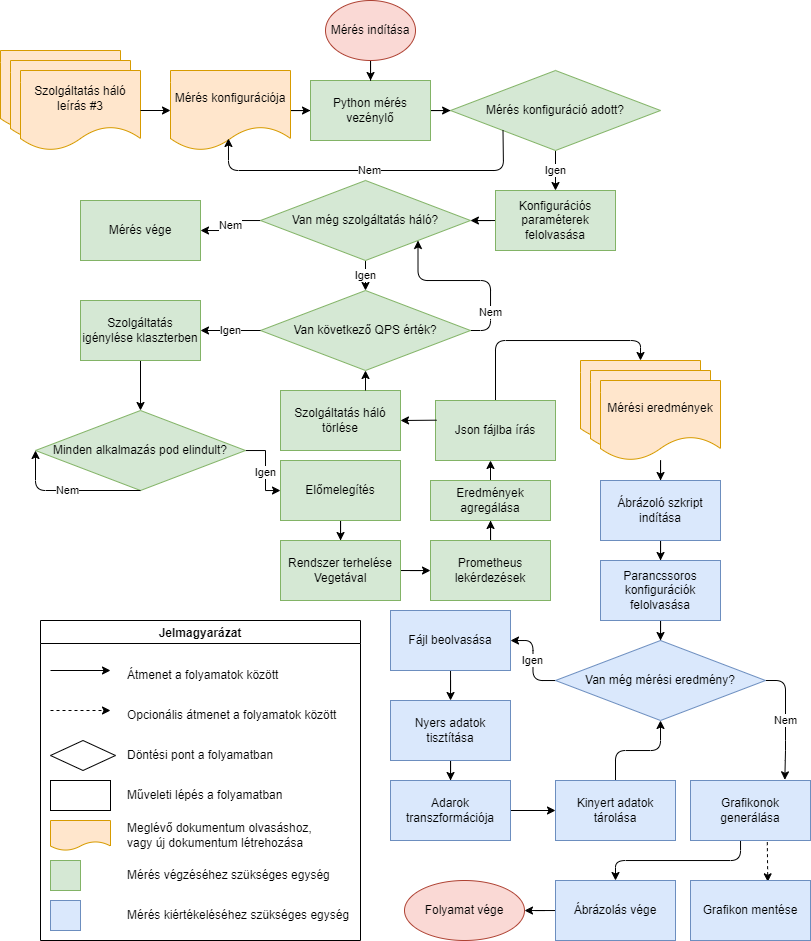
\includegraphics[width=150mm, keepaspectratio]{figures/measurement_and_draw_workflow.png}
\caption{Szimuláció futtatásának és kiértékelésének lépései}
\label{fig:measurement_and_draw_workflow}
\end{figure}

